% !TEX encoding = UTF-8 Unicode
% !TEX TS-program = xelatex

\documentclass{article}
	\usepackage[cm]{fullpage}
	\usepackage{fontspec}
	\setmainfont{SourceCodePro-Regular}
	\usepackage{tikz}
	\usepackage{listings}
\begin{document}

	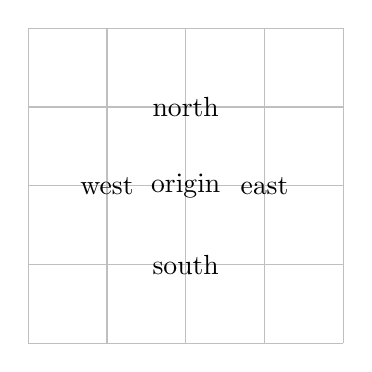
\begin{tikzpicture}
		\draw [lightgray] (-2, -2) grid (2, 2);
		                         \node at (0, 1) {north};
		\node at (-1, 0) {west}; \node at (0, 0) {origin}; \node at (1, 0) {east};
		                         \node at (0, -1) {south};
	\end{tikzpicture}

\lstset{language=[latex]tex,tabsize=4}
\lstset{moretexcs={draw}}



%%%%%%%%%%%%%%%%%%
\begin{lstlisting}
% !TEX encoding = UTF-8 Unicode
% !TEX TS-program = pdflatex
\documentclass{article}
	\usepackage{tikz}
\begin{document}
	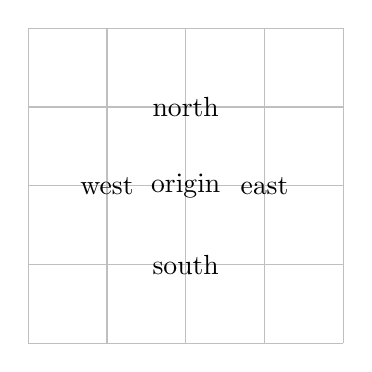
\begin{tikzpicture}
		\draw [lightgray] (-2, -2) grid (2, 2);
		                     \node at(0,1){north};
		\node at(-1,0){west};\node at(0,0){origin};\node at(1,0){east};
		                     \node at(0,-1){south};
	\end{tikzpicture}
\end{document}
\end{lstlisting}
%%%%%%%%%%%%%%%%



\end{document}